\documentclass[a4paper, 12pt]{article}
\usepackage[a4paper,top=1.5cm, bottom=1.5cm, left=1cm, right=1cm]{geometry}
\usepackage{cmap}					
\usepackage{mathtext} 				
\usepackage[T2A]{fontenc}			
\usepackage[utf8]{inputenc}			
\usepackage[english,russian]{babel}
\usepackage{multirow}
\usepackage{graphicx}
\usepackage{wrapfig}
\usepackage{tabularx}
\usepackage{float}
\usepackage{longtable}
\usepackage{hyperref}
\hypersetup{colorlinks=true,urlcolor=blue}
\usepackage[rgb]{xcolor}
\usepackage{amsmath,amsfonts,amssymb,amsthm,mathtools} 
\usepackage{icomma} 
\usepackage{euscript}
\usepackage{mathrsfs}
\usepackage{enumerate}
\usepackage{caption}
\usepackage{enumerate}
\mathtoolsset{showonlyrefs=true}
\usepackage{graphicx}
\usepackage{caption}
\usepackage{subcaption}
\usepackage{amsthm}
\usepackage[europeanresistors, americaninductors]{circuitikz}
\DeclareMathOperator{\sgn}{\mathop{sgn}}
\newcommand*{\hm}[1]{#1\nobreak\discretionary{}
	{\hbox{$\mathsurround=0pt #1$}}{}}

%%% Заголовок

\title{\textbf{Определение теплоты испарения жидкости (2.5.1)}}
\author{Манро Эйден}
\date{}

\begin{document}

\maketitle

\begin{center}
    \section*{Введение}
\end{center}

\noindent \textbf{Цель работы:} 1) измерение давления насыщенного пара жидкости при разной температуре; 2) вычисление по полученным данным теплоты испарения с помощью уравнения Клапейрона-Клаузиуса. 
\bigskip

\noindent \textbf{Оборудование:} термостат; герметический сосуд, заполненный исследуемой жидкостью; отсчётный микроскоп. 

\bigskip

\subparagraph*{Теоретические сведения.} 

Испарением называется переход вещества из жидкого в газообразное состояние. Оно происходит на свободной поверхности жидкости. При испарении с поверхности вылетают молекулы, образую над ней пар. Для выхода из жидкости молекулы должны преодолеть силы молекулярного сцеления. Кроме того, при испарении совершается работа против внешнего давления $P$, поскольку объём жидкости меньше объёма пара. Не все молекулы жидкости способны совешить эту работу, а только те из них, кто обладает достаточной кинетической энергией. Поэтому переход части молекул в пар приводит к обеднению жидкости быстрыми молекулами, т. е. к её охлаждению. Чтобы испарение проходило без изменения температуры, к жидкости нужно подводить тепло. Количество теплоты, необходимое для изотермического испарения одного моля жидкости при внешнем давлении, равном упругости её насыщенных паров, называется её молярной теплотой испарения (парообразования). 

Теплоту парообразования жидкостей можно измерить непосредственно при помощи калориметра. Такой метод, однако, не позволяет получить точных результатов из-за неконтролируемых потерь тепла, которые трудно сделать малыми. В настоящей работе для определения теплоты испарения применен косвенный метор, основанный на формуле Клапейрона-Клаузиуса: 

\bigskip

\begin{equation} \label{kk}
 	\dfrac{dP}{dT}= \dfrac{L}{T(V_2 - V_1)}. 
\end{equation}

\bigskip

Здесь  $P$ -- давление насыщенного пара жидкости при температуре  $T$,  $T$ -- абсолютная температура жидкости и пара, $L$ -- теплота испарения жидкости,  $V_1$ -- объём шара,  $V_2$ -- объём жидкости. Найдя из опыта  $dP/dT, T, V_2$ и $V_1$, можно определить $L$ путём рассчёта. Величины $L, V_2$ и $V_1$ в формуле \eqref{kk} должны относиться к одному и тому же количеству вещества; мы будем относить их к одному молю. 

В нашем приборе измерения проводятся при давлениях ниже атмосферного. В этом случае задача существенно упрощается. 

В таблице для ряда жидкостей приведены: температура, при которой давление насыщенных паров равно атмосферному, величины $V_1$ и $V_2$, входящие в \eqref{kk}, а так же константы $a$ и $b$ в уравнении Ван-дер-Ваальса. 

\bigskip

\begin{center}
	\begin{tabular}{|c|c|c|c|c|c|c|} 
	\hline
	& $T_{\text{кип}}$,&$ V_1$, &$ V_2 , $&$ b$,& $ a$, & $a / V^2$, \\
	Вещество&  & $10^{-6}$ &$10^{-3}$&$10^{-6}$&& \\
	& К &$\frac{\text{м}^3}{\text{моль}} $&$\frac{\text{м}^3}{\text{моль}} $&$\frac{\text{м}^3}{\text{моль}} $&$\frac{\text{Па} \cdot \text{м}^6}{\text{моль}^2} $ &кПа\\ 
	\hline 
	Вода & 373 & 18 & 31 & 26 & 0,4& 0,42 \\ 
	CCl$_4$ & 350 & 97 & 29 & 126 & 1.95 & 2,3 \\ 
	Этиловый эфир & 307 & 104 & 25 & 137 & 1,8 & 2,9 \\ 
	Этиловый спирт & 351 & 58 & 29 & 84 & 1,2 & 1,4 \\ \hline
	\end{tabular}
\end{center}

\bigskip

Из таблицы видно, что $V_1$ не превосходит $0,5 \%$  от  $V_2$. При нашей точности опытов величиной $V_1$ в \eqref{kk} можно пренебречь. 

Обратимся теперь к $V_2$, которое в дальнейшем будем обозначать просто $V$. Объём $V$  связан с давлением и температурой уравнением Ван-дер-Ваальса:

\bigskip

\begin{equation} \label{vv}
	\left(P + \dfrac{a}{V^2}\right)\left(V - b\right)= RT.
\end{equation}

\bigskip

Из таблицы можно видеть, что $b$ одного порядка с $V_1$. В уравнении Ван-дер-Ваальса величиной $b$ следует пренебречь. Пренебрежение членом $a/V^2$  по сравнению с $P$ вносит ошибку меньше $3\%$ . При давлении ниже атмосферного ошибки становятся ещё меньше. Таким образом, при давлениях ниже атмосферного уравнение Ван-дер-Ваальса для насыщенного пара мало отличается от уравнения Менделеева-Клапейрона. Положим поэтому

\bigskip

\begin{equation} \label{ig}
	V = \frac{RT}{P}.
\end{equation}

\bigskip

Подставляя \eqref{ig} в \eqref{kk}, пренебрегая $V_1$ и разрешая уравнение относительно $L$, найдём 

\bigskip

\begin{equation} \label{res}
	L = \frac{RT^2}{P}\frac{dP}{dT}=-R\frac{d(\ln P)}{d(1/T)}
\end{equation}

\bigskip

Эта формула является окончательной. 

В нашем опыте температура жидкости измеряется термометром, давление пара определяется  при помощи манометра, а производная $dP / dT$ $d(\ln P) / d(1 / T) $ находятся графически как угловой коэффициент касательной к кривой $P(T)$ или соответственно к кривой, у которой по оси абсцисс отложено $1/T$, а по оси ординат $\ln P$. 

\subparagraph*{Экспериментальная установка.} Cхема установки изображена на рис. 1 Наполненный спиртом в нашем случае резервуар 1 играет роль термостата. Нагревание термостата производится спиралью 2, подогреваемой электрическим током. Для охлаждения спирта в термостате через змеевик 3 пропускается водопроводная вода. Спирт в термостате перемешивается воздухом, поступающим через трубку 4. Температура спирта измеряется термометром 5. В термостат погружен запаянный прибор 6 с исследуемой жидкостью. Над ней находится насыщенный пар (перед заполнением прибора воздух из него был откачан). Давление насыщенного пара определяется по ртутному манометру, соединённому с исследуемым объёмом. Отсчёт показаний манометра производится при помощи микроскопа. 

Описание прибора указывает на второе важное преимущество предложенного косвенного метода измерения $L$ перед прямым. При непосредственном измерении теплоты испарения опыты нужно производить при неизменном давлении, и прибор может быть не запаян. При этом невозможно обеспечить такую чистоту и неизменность экспериментальных условий, как при нашей постановке опыта. 

Описываемый прибор обладает важным недостатком: термометр определяет температуру термостата, а не исследуемой жидкости (или её пара). Эти температуры близки друг к другу лишь в том случае, если нагревание происходит достаточно медленно. Убедиться в том, что темп нагревания не является слишком быстрым, можно, сравнивая результаты, полученные при нагревании и при остывании прибора. Такое сравнение необходимо сделать. Для ориентировки укажем, что температуру воды в калориметре следует менять не быстрее, чем на $2^{\circ}$С в течение 1---3 минут. 

\begin{figure}[h]	\label{plan1}
	
	\center{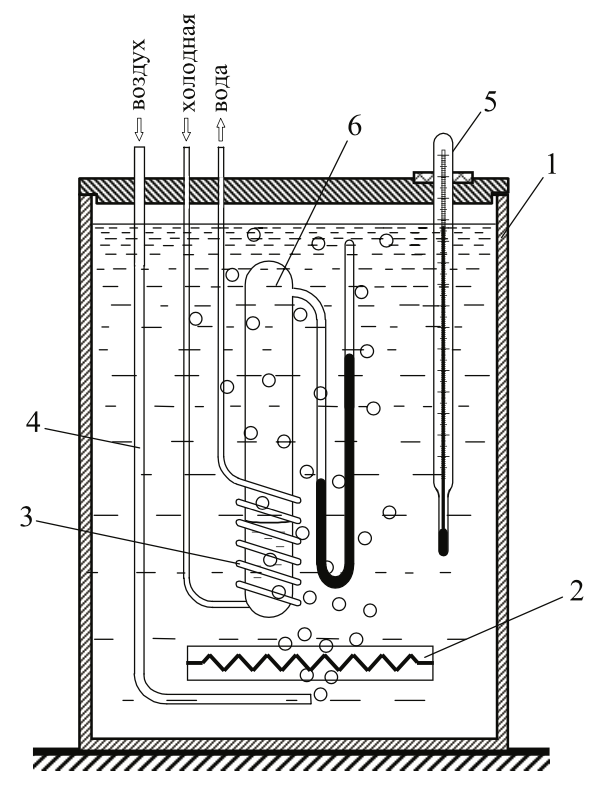
\includegraphics[width= 0.5\linewidth]{IMG_2.jpg}}
	\caption{Схема установки для определения теплоты испарения}

\end{figure}	

\begin{figure}[b!]	\label{plan2}
	
	\center{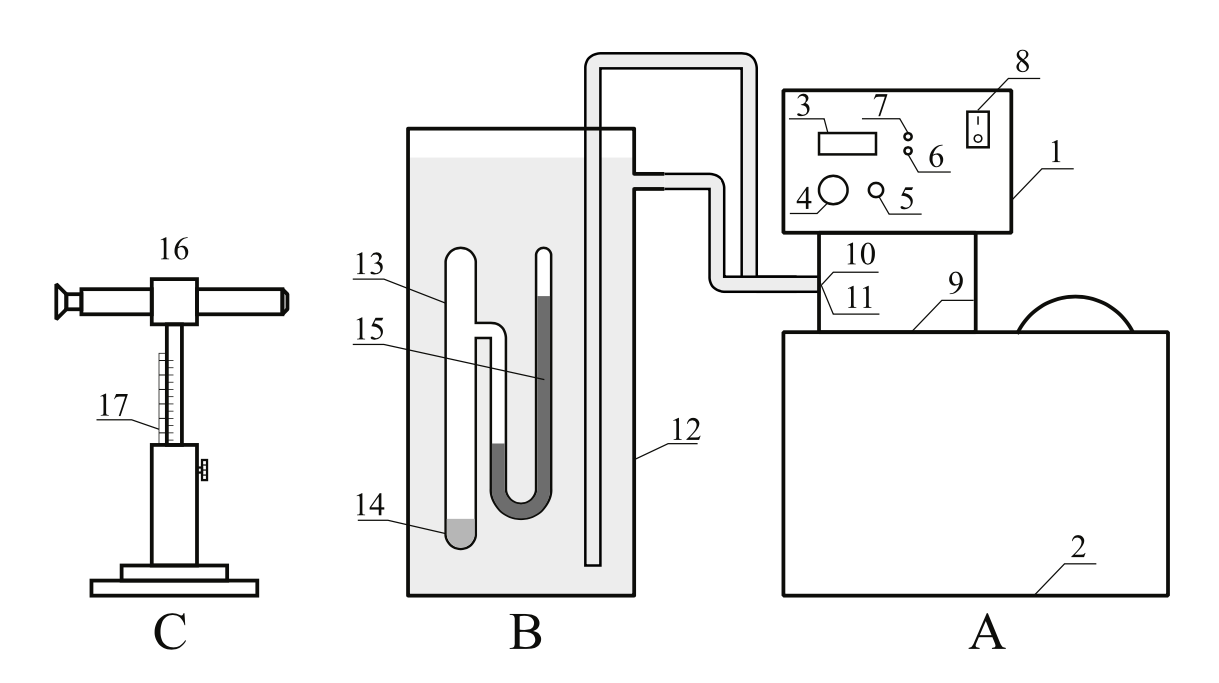
\includegraphics[width=1 \linewidth]{IMG_1.jpg}}
	\caption{Более полная схема установки}

\end{figure}

\newpage

\subparagraph*{Погрешности.}

\begin{itemize}
	\item $ \sigma_{\ln{P}} = \dfrac{\sigma P}{P} = 9,5 \; \cdot \; 10^{-4} \;$
	\item $ \sigma_{P} = 2,66 \; \text{Па}$
	\item $ \sigma_{\frac{1}{T}} = 1 \; \cdot \; 10^{-6} \; K  $
	\item $ \sigma_{t} = 0,1 \; ^{\circ}C $ 
\end{itemize}

\begin{center}
	\section*{Ход работы}
\end{center}

\subparagraph*{1.} Измерим высоты, на которых расположены мениски в ртутном U-образном манометре с помощью микроскопа и температуру по  индикаторному табло. Вычислим разность уровней $\Delta h$. Данные занесём в Таблицу 1. 

\subparagraph*{2.} Продолжая повышать температуру нагреем жидокость до температуры $\approx 40^{\circ}$С,
через каждыйе 2 градуса будем проводить те же измерения, занося данные в Таблицу 1. 

\begin{table}[h!] 
	\caption{Экспериментальные данные}
	\begin{center}
	\begin{tabular}{|*{2}{l|}}
		\hline 
		$t$,&$\Delta h$,      \\ 
		$^{\circ}$C&\text{мм} \\ \hline

		25,12 & 57,79   	  \\ \hline 
		27,01 & 63,89   	  \\ \hline 
		29,01 & 71,55   	  \\ \hline 
		31,00 & 81,20   	  \\ \hline 
		33,00 & 90,39   	  \\ \hline 
		35,01 & 100,21  	  \\ \hline 
		37,00 & 112,62  	  \\ \hline 
		39,00 & 124,57  	  \\ \hline 
		40,00 & 130,25  	  \\ \hline \hline
		37,01 & 109,06  	  \\ \hline 
		34,00 & 93,41   	  \\ \hline 
		31,00 & 79,34   	  \\ \hline 
		28,00 & 68,25   	  \\ \hline 
		25,00 & 58,50   	  \\ \hline 

	\end{tabular}
	\end{center}
\end{table}


\end{document}
